

%\documentclass[runningheads,a4paper]{llncs}
%%\documentclass{llncs}
%\usepackage{amssymb}
%\usepackage{algorithm}
%\usepackage{algorithmic}
%\usepackage{dsfont}
%\usepackage{amsmath}
%\setcounter{tocdepth}{3}
%\usepackage{booktabs}
%\usepackage{multirow}
%\usepackage{graphicx}
%\usepackage{color}
%\usepackage[table]{xcolor}
%
%\usepackage{url}
%\urldef{\mailsa}\path|{agutierrez,eligius,igarciaf}@uma.es|
%\urldef{\mailsb}\path|gloriaortega@ual.es|
%\urldef{\mailsc}\path| {karin.pauls,rene.haijema}@wur.nl|
%\newcommand{\keywords}[1]{\par\addvspace\baselineskip
%\noindent\keywordname\enspace\ignorespaces#1}
%
%\begin{document}
%
%\mainmatter  % start of an individual contribution
%
%% first the title is needed
%\title{On Computing Order Quantities for Perishable Inventory Control with Non-Stationary Demand}
%
%% a short form should be given in case it is too long for the running head
%\titlerunning{On computing order quantities}
%
%% the name(s) of the author(s) follow(s) next
%%
%% NB: Chinese authors should write their first names(s) in front of
%% their surnames. This ensures that the names appear correctly in
%% the running heads and the author index.
%%
%\author{Alejandro G. Alcoba \inst{1}
%\and Eligius M.T. Hendrix \inst{1}
%\and Inmaculada Garc\'ia\inst{1}
%\and Gloria Ortega \inst{2}
%\and Karin G.J. Pauls-Worm \inst{3}
%\and Rene Haijema \inst{3}}
%%
%\authorrunning{Alejandro G. Alcoba et al.}
%
%
%
%\institute{
%            Computer Architecture, Universidad de M{\'a}laga\\
%             \mailsa
%            \and Informatics, Univ. of Almer\'ia, Agrifood Campus of Int. Excell., ceiA3\\
%            \mailsb
%           \and Operations Research and Logistics, Wageningen University\\
%            \mailsc
%}
%
%
%\maketitle
%
%%---------------------------------------------------------------------------
%\begin{abstract}
%The determination of order quantities in an inventory control problem of perishable products with non-stationary demand can be formulated as a Mixed Integer Nonlinear Programming problem (MINLP). One challenge is to deal with the $\beta$-service level constraint in terms of the loss function. This paper studies the properties of the optimal solution and derives specific algorithms to determine optimal quantities.
%
%
%\keywords{Inventory control, Perishable products, MINLP,  loss function, Monte Carlo}
%% \PACS{PACS code1 \and PACS code2 \and more}
%% \subclass{MSC code1 \and MSC code2 \and more}
%\end{abstract}

\chapter{On computing order quantities for perishable inventory control with non-stationary demand} % top level followed by section, subsection
\label{Chap:iccsa2015}

\ifpdf
\graphicspath{{X/figures/PNG/}{X/figures/PDF/}{X/figures/}}
\else
\graphicspath{{X/figures/EPS/}{X/figures/}}
\fi

%-------------------------------------------------------------------------------
\section{Introduction}\label{sec:intro}
The basis of our study is a fill rate variant of a Stochastic Programming (SP) model presented in \cite{PAULS14} for a practical production planning problem over a finite horizon of $T$ periods of a perishable product with a fixed shelf life of $J$ periods. Items of age $J$ cannot be used in the next period and are considered waste. Demand is stochastic and non-stationary, as it changes over time. 
To keep waste due to out-dating low, one issues the oldest product first, i.e. FIFO  (first in, first out) issuance. Literature provides many ways to deal with perishable products, order policies and backlogging, e.g. \cite{hedjar2004,kurawarwala96,Silver98}. The model we investigate aims to guarantee a $\beta$-service level constraint; the supplier guarantees expected shortage not to exceed $(1-\beta)\%$ of the expected demand for every period. Not fulfilled demand is lost.

The solution for such a model is a so-called order policy.
We consider a policy with a list of order periods $Y$ with order quantities  $Q_t$. The question is to derive a set of order quantities that leads to minimum cost and fulfils the service level constraint.

Section \ref{sec:model} introduces the model under study. Properties of the order quantities are studied in Section \ref{sec:rcot}. Section \ref{sec:alg} then describes several algorithms to determine solutions, including an optimal one. Sections \ref{sec:parameters} and \ref{sec:exp} analyse the effect of the value of the parameters of the objective function on the optimal delivery orders. Finally, Section \ref{sec:conclusionsICCSA} concludes and summarizes the findings.



\section{Stochastic Programming Model}
\label{sec:model}

The model describes the inventory development over $T$ periods of products with $J$ periods of shelf life, where $t$ is the time index and $j$ is the age of the product in inventory. The stochastic demand implies that the model has random inventory variables $\boldsymbol{I}_{jt}$ apart from the initial fixed levels $I_{j0}$. The model has to keep track of the lost sales $\boldsymbol{X}_t$ in periods where demand exceeds the available amount of product. Moreover, typical is the amount of product that perishes and becomes waste, $\boldsymbol{I}_{Jt}$. In the notation, %$P(.)$ denotes a probability to express the chance constraints and
$E(.)$ is the expected value operator. Moreover,  we use $x^+=max\{x,0\}$. A formal description of the SP model from \cite{PAULS14} is given.\\

\smallskip\noindent\emph{Indices}\\
\begin{tabular}{ll}
$t$ & period index, $t=1,\ldots,T$, with $T$ the time horizon\\
$j$ & age index, $j=1,\ldots,J$, with $J$ the fixed shelf life\\
\end{tabular}


\smallskip\noindent\emph{Data}\\
\begin{tabular}{ll}
$\boldsymbol{d}_t$ &
normally distributed demand with mean value $\mu_t>0$ and variance  $(cv\times \mu_t)^2$\\
& where $cv$ is a given coefficient of variation.\\
$k$ & fixed ordering cost, $k>0$\\
$c$ & unit procurement cost, $c>0$\\
$h$ & unit inventory cost, $h>0$\\
$w$ & unit disposal cost, is negative when having a salvage value, $c>-w$\\
$\beta$ & service level, $0<\beta<1$
\end{tabular}

%\noindent 5pt

\smallskip\noindent\emph{Variables}\\
\begin{tabular}{ll}
$Q_t \ge 0$ & ordered and delivered quantity at the beginning of period $t$\\
$Y_t \in \{0,1\}$ & setup of order\\
$\boldsymbol{X}_t$ & lost sales in period $t$\\
$\boldsymbol{I}_{jt}$ & inventory of age $j$ at end of period $t$, initial inventory fixed  $I_{j0}=0$,\\
 & $\boldsymbol{I}_{jt} \ge 0$ for $j=1,\ldots,J$.\\
\end{tabular}

\smallskip\noindent
The total expected costs over the finite horizon is to be minimized.

\begin{equation}
\label{eq:objICCSA}
f(Q)=\sum_{t=1}^T \left(C(Q_t) + E\left(h\sum_{j=1}^{J-1} \boldsymbol{I}_{jt}  +w\boldsymbol{I}_{Jt}\right)\right),
%\sum_{t=1}^T g(Q_t) + E\left(h\sum_{t=1}^T \sum_{j=1}^{J-1} \boldsymbol{I}_{jt}^+ +w\boldsymbol{I}_{Jt}\right)=\sum_{t=1}^T g(Q_t) + E\left(h\sum_{j=1}^{J-1} \boldsymbol{I}^+_{jt}  +w\boldsymbol{I}_{Jt}\right),
\end{equation}
where procurement cost is given by the function
\begin{equation}
\label{eq:procICCSA}
C(x) = k+cx, \ \ \text{if} \ \ x>0,\ \text{and}\ \ C(0)=0 .
\end{equation}
%
The FIFO dynamics of inventory of items of  age $j$ starts by defining waste ($j=J$)
\begin{equation}
\label{eq:invWasteICCSA}
\boldsymbol{I}_{Jt}=(\boldsymbol{I}_{J-1,t-1} - \boldsymbol{d}_t)^+, \ t=1,\ldots,T
\end{equation}
followed by the inventory of items with age $1<j<J$ that still can be used in the next period:
\begin{equation}
\label{eq:inv2ICCSA}
\boldsymbol{I}_{jt}= \left(\boldsymbol{I}_{j-1,t-1} - (\boldsymbol{d}_t-\sum_{i=j}^{J-1}\boldsymbol{I}_{i,t-1})^+\right)^+, \ t=1,\ldots,T, j=2,\ldots,J-1 .
\end{equation}
%
and finally the incoming and freshest products, $j=1$:
%
\begin{equation}
\label{eq:inv1ICCSA}
\boldsymbol{I}_{1t}= \left(Q_t - (\boldsymbol{d}_t-\sum_{j=1}^{J-1}\boldsymbol{I}_{j,t-1})^+\right)^+, \ t=1,\ldots,T.
\end{equation}
%
Lost sales for period $t$ is defined by
%
\begin{equation}
\label{eq:lostsalesICCSA}
\boldsymbol{X}_t=\left(\boldsymbol{d}_t-\sum_{j=1}^{J-1}\boldsymbol{I}_{j,t-1}-Q_t\right)^+.
\end{equation}
%
The service level constraint for every period is
\begin{equation}
\label{eq:chanceICCSA}
E \left(\boldsymbol{X}_t\right) \le (1-\beta) \mu_t, \ t=1,\ldots,T.
\end{equation}
%
Notice that given the stochastic variables of demand, the expectation of lost sales only depends on the ordered quantities $Q: (Q_1,\ldots, Q_T)$. For a MINLP approach, we can also express these constraints as follows
%
\begin{equation}
\label{eq:defg}
g_t(Q)=E \left(\boldsymbol{X}_t\right) - (1-\beta)\mu_t\le 0,\ t=1,\ldots,T.
\end{equation}
%
We consider a simple order policy, where the decision maker should provide an integer vector $Y=(Y_1,\ldots,Y_T)\subset \{0,1\}^T$ of order periods and order quantities $Q_t$ with $t=1,\ldots,T$ where $Y_t=0$ implies $Q_t=0$. Finding the best values of the (continuous) order quantities $Q_t$ and the corresponding optimal (integer) order timing $Y$ can be considered a MINLP problem. In summary, we have a $MINLP (Q)$ problem:
$\min_Q f(Q)$
subject to the inventory development (\ref{eq:invWasteICCSA}), (\ref{eq:inv2ICCSA}), (\ref{eq:inv1ICCSA}), (\ref{eq:lostsalesICCSA}) and $g_t(Q)\le 0,\ t=1,\ldots,T$.




\section{Replenishment Cycles and Basic Order Quantities}
\label{sec:rcot}
%
We study several theoretical properties of the order quantities $Q$ and the list of order periods $Y$. We first focus on the concept of replenishment cycles in Section \ref{sec:repl} and determine in which cases a so-called basic order quantity defines the optimal order quantity in Section \ref{sec:safe}. Section \ref{sec:nlp} then derives properties of the optimal quantities given a timing vector $Y$, which can be used in the design of specific algorithms in Section \ref{sec:alg}.


\subsection{Feasible Replenishment Cycles}
\label{sec:repl}

Literature on inventory control (e.g. \cite{Silver98}) applies the concept of a replenishment cycle, i.e. the length of the period $R$ for which the order of size $Q$ is meant. For stationary demand, the replenishment cycle is fixed, but for non-stationary demand the optimal replenishment cycle may depend on the period.
 \begin{defn}
 \label{def:A}
Given a list of order periods $Y\in \{0,1\}^T$ and $M=\sum_{t=1}^T Y_t$. The order timing vector $A \in \mathbb{N}^M$ for $Y$ gives the periods $A_i< A_{i+1}$ where  $Y_{A_i}=1$.
\end{defn}
%
\begin{defn}
 \label{def:R}
Given a list of order periods $Y\in \{0,1\}^T$ with total number of orders $M=\sum_{t=1}^T Y_t$. Replenishment cycle $R_i=A_{i+1}-A_i, \ i=1,\ldots,M-1$ and $R_M=T-A_M+1$.
\end{defn}
Notice that for the perishable case with a shelf life $J$, to fulfil the service level constraint, practically the replenishment cycle cannot be larger than the shelf life $J$; so $1 \le R_i \le J$.
\begin{lemma}
\label{lem:Y}
Let $Y$ be an order timing vector of the SP model, i.e. $Y_t=0 \Rightarrow Q_t=0$. $Y$ provides an infeasible solution of the SP model, if it contains more than $J-1$ consecutive zeros.
\end{lemma}
This means that a feasible order timing vector $Y$ does not contain a consecutive series with more than $J-1$ zeros.

\begin{defn}
Let $F_T$ be the set of feasible order timing vectors $Y$ of length $T$.
\end{defn}

For the given model the number of elements $|F_T|$, for $T\leq J$ is equal to $2^{T-1}$. Given the assumption of zero starting inventory, an element $Y\in F_T$ must start with $Y(1)=1$, otherwise demand will not be satisfied for the first period. From here, any combination is valid, since there are no more than $J-1$ elements to consider. The case $T=J+1$ is slightly different: for the first period again $Y(1)=1$ is needed, and for the rest of elements there are $2^J$ possible cases, and only the one with $J$ zeros is not feasible, so $|F_{J+1}|=2^J-1$.

For $T>J+1$ the number of feasible series can be derived recursively according to the following proposition.
\begin{proposition}
\label{prop:numberfeasible}
The number of elements $|F_T|$ of the set $F_T$ of feasible order timings of $T$ periods and a shelf life $J$ with $J+1<T$ follows the recursive rule
\begin{figure}[h]
\centering
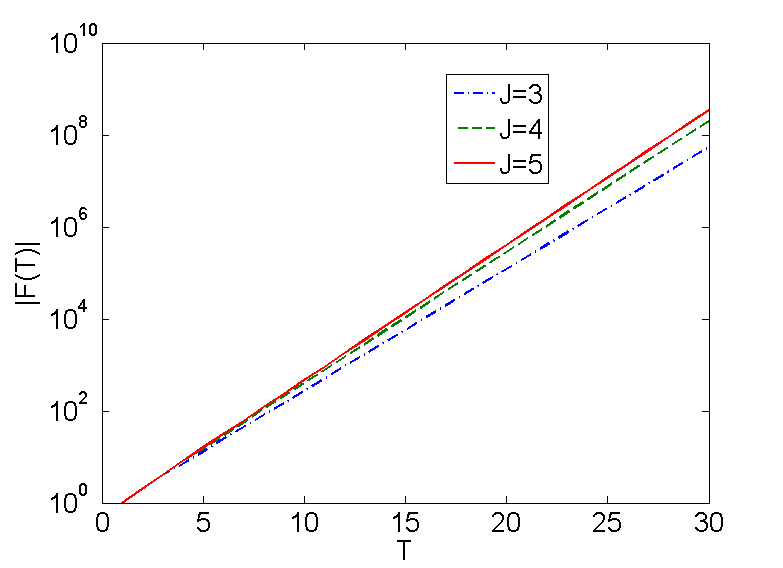
\includegraphics[scale=0.4]{iccsa2015/figures/numberfeasiblelogy.png} % escala semilogaritmica
%\includegraphics[scale=0.5]{numberfeasible.png} %escala normal (equi)
\caption{ $|F(T)|$ as a function of $T$ and several values of the shelf life $J$.}
\label{fig:numberfeasible}
\end{figure}

\begin{equation}
\label{eq:numberfeasibleY(T)}
|F_{T+1}|= 2|F_{T}| -|F_{T-J}|
\end{equation}
with the initial terms  $|F_{t}|=2^{t-1}, \  t<J+1$, and  $|F_{J+1}|=2^J-1 $
\end{proposition}

\begin{proof}
Consider $p=(p_1,\ldots,p_{T})\in F_{T}$, then obviously $(p_1,\ldots,p_{T},1)\in F_{T+1}$. We now focus on the case of $(p,0)=(p_1,\ldots,p_{T},0)$. Its feasibility is determined by the values of $p_{T-(J-2)},\ldots, p_{T-1},p_T$. Let $\boldsymbol{0}$ be now an all zeros vector with $J-1$ elements. If $(p_{T-(J-2)},\ldots, p_{T-1},p_T)=\boldsymbol{0}$, then $(p,0)$ is not feasible. But how many feasible $p\in F_{T}$ exist with this feature?

Given $(p_{T-(J-2)},\ldots, p_{T-1},p_T)=\boldsymbol{0}$ and $p\in F_{T}$, we must have $p_{T-J+1}=1$. There are $|F_{T-J}|$ feasible timing vectors $(p_1,\ldots,p_{T-J})$ with $(p_1,\ldots,p_{T-J},1,\boldsymbol{0})$  feasible and  $(p_1,\ldots,p_{T-J},1,\boldsymbol{0},0)$ infeasible.
From this follows the final result, $|F_{T+1}|= 2|F_{T}| -|F_{T-J}|$.
%\qed
\end{proof}




The proof of Proposition~\ref{prop:numberfeasible} gives a constructive method to determine all feasible policies recursively. Moreover, (\ref{eq:numberfeasibleY(T)}) shows that the space of feasible policies grows exponentially with $T$ as illustrated in Figure~\ref{fig:numberfeasible}.



\subsection{Basic Order Quantities}
\label{sec:safe}
We focus now on the minimum order quantity at period $t\in \{1,\ldots,T\}$  to cover demand for the next $r$ periods $t, t+1,\ldots, t+r-1$ that is just sufficient according to the service level constraint where at period $t$ no older items are in stock.
\begin{figure}[h]
\centering
%\includegraphics[scale=0.5]{lossfunction.png}
\includegraphics[scale=0.4]{iccsa2015/figures/lossfunFig.png}
%\includegraphics[scale=0.5]{lossfunFig.pdf}
\caption{One period loss function $E(X|Q)$ for $\boldsymbol d \sim N(1950,0.25\cdot1950)$ and corresponding basic order quantity $q$: $E(X|q)=(1-\beta)\mu$}
\label{fig:lossfunFig}
\end{figure}
\begin{defn}
Basic order quantity $\overline Q_{r,t}$ is the amount for period $t$ that fulfils constraint (\ref{eq:chanceICCSA}) for the next $r$ periods: $t,t+1,\ldots,t+r-1$.
\end{defn}
We first consider $\overline Q_{1t}$. Let the replenishment cycle be one period $R=1$, zero inventory and $q$ the order quantity. In this case, lost sales $X$ from expression (\ref{eq:lostsalesICCSA}) can be simplified to:
%
\begin{equation}
\boldsymbol{X}=\left(\boldsymbol{d}-q\right)^+ .
\end{equation}
Let $\varphi$ be the density function (pdf) of $\boldsymbol d$ and $\Phi$ be the corresponding cumulative distribution function (cdf).
%
%
Then the so-called loss function expressing the expected lost sales as a function of $q$ is
%
\begin{equation}
L(q) = E(\boldsymbol{X})=E\left((\boldsymbol{d}-q)^+\right)= \int\limits_{q}^{\infty} (x-q)\varphi(x)dx,
\end{equation}
%
where the symbol $x$ is used here as the argument in the integral. The cost function (\ref{eq:objICCSA}) is monotonously increasing in the order quantity $q$ and $L(q)$ decreases, so constraint (\ref{eq:chanceICCSA}) is binding for the optimal value of $q$ such that $L(q) = (1-\beta) \mu$ as illustrated in Figure~\ref{fig:lossfunFig}. Since demand is normally distributed, there is no closed-form expression for the first order loss function.  Some approximations for the loss function can be found in  \cite{kurawarwala96},\cite{Rossi14},\cite{DeSchrijver20121375},\cite{Waissi199691}. From a root-finding perspective, there are several ways to proceed (see \cite{HENTO10}). For instance, one can use the derivative of loss function  $L'(q)=\int\limits_{-\infty}^{q}\varphi(x)dx - 1 = \Phi(q) - 1$ to approximate $q$ using \emph{Newton-Raphson} method. The following theoretical result shows that for the described model, the determination of $q$ has to be done only once.
%
\begin{lemma}
\label{lem:q1}
Let $\boldsymbol{d}\sim N(\mu,cv\times \mu)$ and $\varphi$ be the pdf and $\Phi$ the cdf of the standard normal distribution. The solution of  $L(q) = (1-\beta) \mu$ fulfils $q=\mu(1+cv\times\hat x)$ where $\hat x$ solves
$\varphi\left(\hat x\right)-\left(1-\Phi\left(\hat x\right)\right)\hat x =\frac{1-\beta}{cv}$.
\end{lemma}
%
\begin{proof}
Using the results in \cite{Rossi14} for $\boldsymbol{d}\sim N(\mu,cv\times\mu)$,  the loss function can be expressed as
%
\begin{equation}
\label{eq:rossi}
L(q)=cv\times\mu \left(\varphi\left(\frac{q-\mu}{cv\cdot\mu}\right)-\left(1-\Phi\left(\frac{q-\mu}{cv\cdot\mu}\right)\right)\frac{q-\mu}{cv\cdot\mu}\right) .
 \end{equation}
The Equation $L(q)=(1-\beta)\mu$ substituting $q=\mu(1+cv\times\hat x)$ implies
%
\begin{equation}
\label{eq:rossi2}
 \varphi\left(\frac{q-\mu}{cv\cdot \mu}\right)-\left(1-\Phi\left(\frac{q-\mu}{cv\cdot \mu}\right)\right)\frac{q-\mu}{cv\cdot \mu} =
\varphi(\hat x)-(1-\Phi(\hat x))\hat x =
 \frac{1-\beta}{cv} .
 \end{equation}
%\qed
\end{proof}
%
\begin{figure}[!bt]
\centering
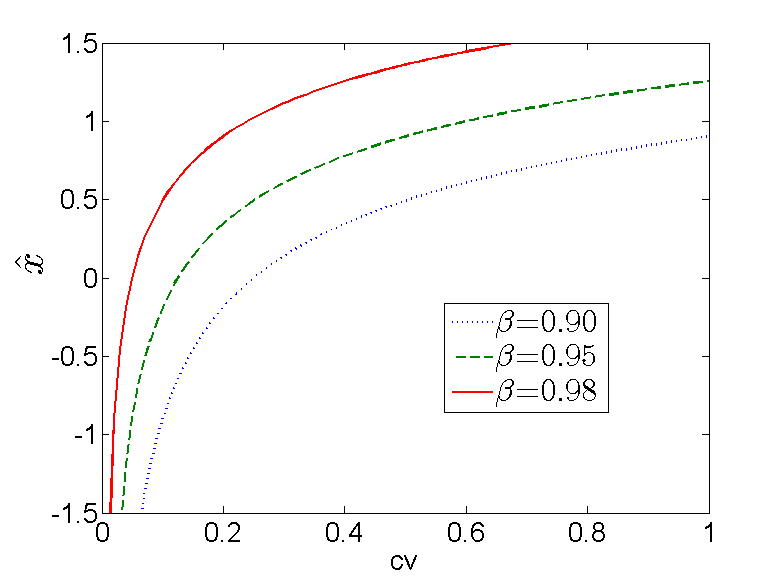
\includegraphics[scale=0.4]{iccsa2015/figures/xhat_ncvnew.png}
%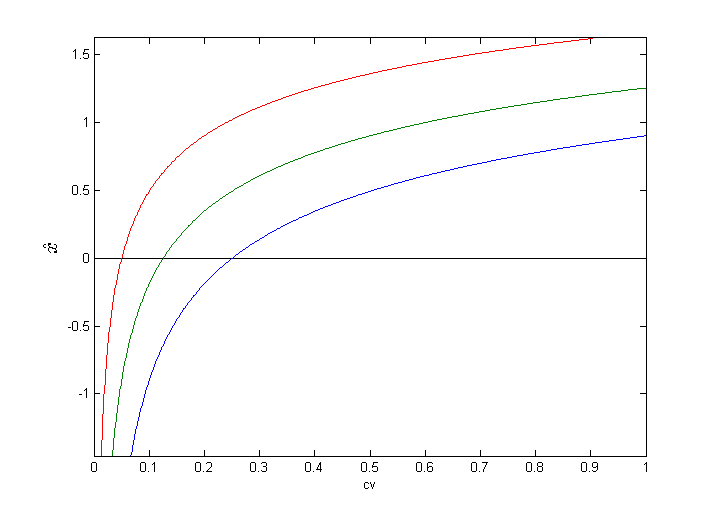
\includegraphics[scale=0.4]{xhat_ncv.pdf}
\caption{Solution $\hat x$ of (\ref{eq:rossi2}) as function of $cv$ for several values of $\beta=0.90, \ 0.95, \ 0.98$ %(blue) $\beta=0.95$ (green) and $\beta=0.98$ (red)
}
\label{fig:xhat_ncv}
\end{figure}
%
The basic order quantity $\overline Q_{1t}= \mu_t(1+cv\times\hat x)$ provides an upper bound on the order quantity $Q_t$ if $R_t=1$, because inventory may be available. Figure~\ref{fig:xhat_ncv} shows the relation of $\hat x$ with parameters $cv$ and $\beta$. Its value indicates how much bigger (smaller if negative) the basic quantity is compared to $\mu$.

The basic order quantities for longer replenishment cycles look more complicated. For instance, $R_t=2$ implies
$$E\left(\boldsymbol{d}_{t+1}-(\overline Q_{2t}-\boldsymbol{d}_{t})^+)\right)^+=(1-\beta)\mu_{t+1} .$$ 
%
These expressions become more cumbersome with the size of the replenishment period. To solve them we need a different approach.
%
Consider a replenishment cycle of $r$ periods, from $t_1$ to $t_2$ with $t_2=t_1+r-1$ and $\boldsymbol{d_{t_1,t_2}} = \boldsymbol {d_{t_1}} + \ldots + \boldsymbol {d_{t_2}}$.  Let $\varphi_{t_1,t_2}$ be the density function (pdf) of $\boldsymbol d_{t_1,t_2}$ and $\Phi_{t_1,t_2}$ be the corresponding cumulative distribution function (cdf). As we are considering that demand is normally distributed, the distribution of $\boldsymbol d_{t_1,t_2}$ is normal as well, with expected value $\mu=\mu_{t_1} + \ldots + \mu_{t_2}$ and $\sigma=cv \sqrt{\mu^2_{t_1} + \ldots+\mu^2_{t_2}}$. Starting with $q$ units at period $t_1$, the expected value of the sum of lost sales from periods $t_1$ to $t_2$, $SL_{t_1,t_2}(q)$ is determined by
\begin{equation}
\label{eq:sumloss}
SL_{t_1,t_2}(q)=E\left(\sum\limits_{i=t_1}^{i=t_2}X_i\right) =E\left((\boldsymbol{d_{t_1,t_2}}-q)^+\right)= \int\limits_{q}^{\infty} (x-q)\varphi_{t_1,t_2}(x)dx.
\end{equation}
Following the considerations in \cite{Rossi14}, $SL_{t_1,t_2}(q)$ can be expressed as
%
\begin{equation}
\label{eq:rossitotloss}
SL_{t_1,t_2}(q)=\mu-q+\sigma\varphi\left(\frac{q-\mu}{\sigma}\right)+\Phi\left(\frac{q-\mu}{\sigma}\right)(q-\mu).
 \end{equation}
% where $\mu=\mu_{t_1} + \ldots + \mu_{t_2}$ and $\sigma=cv \sqrt{\mu^2_{t_1} + \ldots+\mu^2_{t_2}}$.
Now consider the expected lost sales $L_{t_1,t_2}(q)$ in period $t_2$ when $q$ fresh units are available at the beginning of period $t_1$. The quantity follows from subtracting from the expected total lost sales up to period $t_2$ in (\ref{eq:sumloss}) the expected value of total lost sales from periods $t_1$ to $t_2 -1$
\begin{eqnarray}
\label{eq:lostsalesgeneral}
L_{t_1,t_2}(q)&=& SL_{t_1,t_2}(q)- SL_{t_1,t_2-1}(q) = \\ \nonumber
&&=\int\limits_{q}^{\infty} (x-q)\left(\varphi_{t_1,t_2}(x)-\varphi_{t_1,t_2-1}(x)\right)dx.
\end{eqnarray}
To find the value $q_{rt}$ for which the service level constraint is just fulfilled in period $t_2=t+r-1$ when having $q_{rt}$ fresh units at the beginning of period $t$ follows from solving $L(q_{1t})=(1-\beta)\mu_t$ according to Lemma \ref{lem:q1} and for $r>1$ one can solve
\begin{equation}
\label{eq:partialbasic}
SL_{t,t+r-1}(q_{rt})-SL_{t,t+r-2}(q_{rt})=(1-\beta)\mu_{t+r-1}
 \end{equation}
 for $q_{rt}$. The basic order quantity $\overline Q_{rt}$ now follows from taking the maximum of these quantities $\overline Q_{rt}=\max_{j=1,\ldots,r}q_{jt}$, such that the service level constraint is fulfilled in all periods of the replenishment cycle. The values of the basic order quantities in Table %\ref{tab:demand}
 \ref{tab:Ybasicorder} follow from the parameter values in Example \ref{ex:mainexample}.
%%%%%%



\begin{example}
\label{ex:mainexample}

Consider an instance of the problem with $T=12$ periods and shelf life $J=3$. Random variables of demand for every period are expressed in terms of their mean values $\mu_t$ given in last row of Table \ref{tab:Ybasicorder} and the coefficient of variation is given by $cv=0.25$. The required service level is $\beta=95\%$, such that the value of $\hat x$ in Lemma \ref{lem:q1} is $\hat x=0.493$. This value can be used, by Lemma \ref{lem:q1}, to determine the values for $\overline Q_{1t}$ in the first row of Table  \ref{tab:Ybasicorder}. Solving (\ref{eq:partialbasic}) and taking  $\overline Q_{rt}=\max_{j=1,\ldots,r}q_{jt}$ provides values for $\overline Q_{rt}$ for $r>1$ in Table \ref{tab:Ybasicorder}. The values are rounded up.
%
\end{example}



\begin{table}[h]
	\caption{Basic order quantities}
	\label{tab:Ybasicorder}
	\centering
	\resizebox{0.9\columnwidth}{!}{
		\begin{tabular}{@{}lrrrrrrrrrrrr@{}}
			\toprule
			r$\setminus$t        & \multicolumn{1}{c}{1} & \multicolumn{1}{c}{2} & \multicolumn{1}{c}{3} & \multicolumn{1}{c}{4} & \multicolumn{1}{c}{5} & \multicolumn{1}{c}{6} & \multicolumn{1}{c}{7} & \multicolumn{1}{c}{8} & \multicolumn{1}{c}{9} & \multicolumn{1}{c}{10} & \multicolumn{1}{c}{11} & \multicolumn{1}{c}{12} \\ \midrule
			1 & \textbf{898}          & 1067                  & 224                   & 1010                  & 898                   & \textbf{168}          & 730                   & 898                   & \textbf{1010}         & \textbf{336}           & 168                    & 673                    \\
			2 & 1952                  & \textbf{1450}         & 1211                  & \textbf{1925}         & 1225                  & 885                   & \textbf{1618}         & 1898                  & 1458                  & 529                    & \textbf{825}           & 0                      \\
			3 & 2372                  & 2277                  & 2131                  & 2287                  & 1812                  & 1769                  & 2596                  & 2386                  & 1666                  & 1145                   & 0                      & 0                      \\ \midrule
			$\mu_t$  & 800                   & 950                   & 200                   & 900                   & 800                   & 150                   & 650                   & 800                   & 900                   & 300                    & 150                    & 600
		\end{tabular}
	}
\end{table}

\subsection{Optimal Quantities for a Given $Y$}
\label{sec:nlp}
So far, we have described a method to find a feasible $Q$ vector for a given $Y$, using the so called Basic order quantities. Now we can define a method to optimize the objective function (\ref{eq:objICCSA}) subject to a given timing vector $Y$.

We consider now the properties of the MINLP problem described in Section \ref{sec:model}. We first focus on the monotonicity of the objective function in the order quantities when $w>-c$ applies.



\begin{lemma}
\label{lem:finalg}
Given an order timing vector $Y$ with corresponding values $A$ and $M$ according to Definition \ref{def:A}, if $Q^*(Y)$ is an optimal solution of (\ref{eq:objICCSA}),(\ref{eq:procICCSA}),(\ref{eq:invWasteICCSA}), (\ref{eq:inv2ICCSA}), (\ref{eq:inv1ICCSA}), (\ref{eq:lostsalesICCSA}) and (\ref{eq:defg}) with $Q_t= 0$ if $Y_t=0$ then $g_{T}(Q^*)=0$ .%\nonumber.
\end{lemma}
\begin{proof}
Assume $Q^ *$ is optimal and $g_{T}(Q^*)<0$. Due to the inventory dynamics and $g_T$ being a continuous function in its arguments, $\exists \epsilon>0$ such that $Q=Q^*-\epsilon e_{A_M}$ is a feasible solution with $g_{T}(Q)=0$. Due to the FIFO dynamics $I_{jt}(Q)\le I_{jt}(Q^*), j=1,\ldots,J$ and specifically $I_{Jt}(Q^*)-I_{Jt}(Q)\le \epsilon$. As also $\sum Q_t-\sum Q_t^* =\epsilon$ we have that $f(Q)\le f(Q^*)-(c-w)\epsilon < f(Q^*)$ which contradicts $Q^*$ can be optimal with $g_{T}(Q^*)<0$.  
\end{proof}



\begin{proposition}
\label{prop:optimizeY}
Given an order timing vector $Y$ with corresponding values $A$ according to Definition \ref{def:A} and $M=\sum Y_t$.   If $Q^*(Y)$ is an optimal solution of (\ref{eq:objICCSA}),(\ref{eq:procICCSA}),(\ref{eq:invWasteICCSA}), (\ref{eq:inv2ICCSA}), (\ref{eq:inv1ICCSA}), (\ref{eq:lostsalesICCSA}) and (\ref{eq:defg}) with $Q_t= 0$ if $Y_t=0$ then (\ref{eq:defg}) is binding for $t=A_i -1, i=2,\ldots,M$ and $t=T$:
\begin{equation}
\label{eq:optimalQ}
%Q^* =(Q_1^*,\ldots, Q_{T}^*)= min_Q f(Q_1 ,\ldots, Q_{T})\\
 %\text{ s.t. }
 g_{A_2-1}(Q^*) = \ldots = g_{A_M-1}(Q^*)= g_{T}(Q^*)=0 .%\nonumber.
\end{equation}
\end{proposition}
\begin{proof}
Follows from applying the proof of Lemma \ref{lem:finalg} in a sequential way. Lemma \ref{lem:finalg} has shown that $g_{T}(Q^*)=0$. Assume $Q^*$ is optimal with $g_{A_M-1}(Q^*)<0$. As $g_{A_M-1}$ is a continuous function in $Q$, $\exists \epsilon>0$ such that for $Q=Q^*-\epsilon e_{A_{M-1}}$ 
we still have $g_{A_M-1}(Q)<0$. If $R_{M-1}=J$, we have that less items perish at the end of the cycle for $Q$ than for $Q^*$ and therefore $f(Q)<f(Q^*)$ leading to a contradiction.

However, if $R_{M-1}<J$ less inventory $\mathcal{I}(Q)=\sum_{j=R_{M-1}}^{J-1}I_j(Q)$ is available at the end of the cycle and $Q^*_M$ has to be increased to meet the constraint for the last period. \cite{Rossi14} show that the so called complementary loss function $E(\mathcal{I}(Q))$ is strictly convex with partial derivatives less than 1. This implies that $\delta= E(\mathcal{I}(Q^*))-E(\mathcal{I}(Q))<\epsilon$. Consequently there exists a feasible solution $Q^* -\epsilon e_{A_{M-1}} +\delta e_{A_{M}}$ that has lower cost than $Q^*$. This contradicts the assumption. By following this reasoning backward, it is shown that for all periods at the end of a replenishment cycle constraint (\ref{eq:defg}) has to be binding.%\qed   
\end{proof}

Finding (\ref{eq:optimalQ}) implicitly gives a way to determine $Q^*(Y)$. Minimise the quantity of the first cycle up to constraint (\ref{eq:chanceICCSA}) is fulfilled and proceeding with the next cycle until the last one. Notice that given $Y$, the optimal quantities do not depend on the parameter values of the objective function (\ref{eq:objICCSA}).



\section{Algorithms for Generating Order Quantities}
\label{sec:alg}

The derived basic order quantities can now be used to obtain feasible solutions and to improve them towards optimal solutions.

\subsection{Generating a Feasible Solution for a Given $Y$}
Given a list of order periods $Y$ one can determine a feasible solution $Q$ based on $\overline{Q}_{r,t}$.  After determination of $A$ and $R$ from Definitions \ref{def:A} and \ref{def:R}, the appropriate values can be assigned. Example \ref{ex:feasiblesolY} shows a case for a vector $Y$.


\begin{example}
\label{ex:feasiblesolY}
Consider the data and variables of Example \ref{ex:mainexample}. One can determine a feasible solution $Q_t$ for a given timing vector $Y$ using the basic order quantities $\overline Q_{r,t}$. For timing vector $Y=(1,1,0,1,0,1,1,0,1,1,1,0)$, vectors $A$ and $R$ are defined by: $A=(1,2,4,6,7,9,10,11)$ and $R=(1,2,2,1,2,1,1,2)$. Selecting the appropriate basic order quantities results into  $Q=(898,1450,0,$ $1925,0,168,$ $1618,0,1010,$ $336,825,0)$ as illustrated in Table \ref{tab:Ybasicorder}.
\end{example}




\subsection{Generating the Optimal Solution for a Given $Y$}
\begin{algorithm}[h]
	\caption{MinQ($Y$): Optimal order quantity $Q$ for $Y$}
	\label{alg:optimalforYICCSA}
	\begin{algorithmic}[1]
		%\Procedure{MinQ}{$Y$}
        \REQUIRE Orders timing $Y$, fixed shelf life $J$ 
        \ENSURE Optimal order quantity $Q$ for $Y$
        \medskip
		\STATE Determine replenishment periods $A(Y)$, Definition \ref{def:A} 
        \STATE Determine corresponding replenishment cycles $R$, Definition \ref{def:R} 
		\FOR {$i=1$ \textbf{to} $\sum_t Y_t$ } % For every vector of order periods for $Y$
        \IF  { ($A_i=1$ \textbf{or} $A_i -  A_{i-1}=J$) }  %[Inventory is zero] %\hfill \#Inventory is zero
		\STATE $Q_i=Q_{R_i,A_i}$; \label{optimalforY:line:beforeflossICCSA} \hfill \#minimum value for constraint~(\ref{eq:chanceICCSA})
		\STATE  $(z,I_{A_i+R_i-1})=$\textbf{floss}($Q_i,A_i,A_i+R_i-1,0$) \label{optimalforY:line:flossICCSA} \hfill \# Alg. \ref{alg:simulation} updates inventory $I$
		\ELSE
        \STATE $Q_i=$ \textbf{Ordervalue}($A_i,R_i,I_{A_i-1}$) \hfill \# Algorithm~\ref{alg:ordervalueICCSA}
		\ENDIF
		\ENDFOR
		%\EndProcedure
		\vskip 5pt
	\end{algorithmic}
	
\end{algorithm}
The process of optimizing quantities for a timing vector $Y$ is sketched at Algorithm \ref{alg:optimalforYICCSA}. Proposition \ref{prop:optimizeY} shows with (\ref{eq:optimalQ}) that the quantities for the order periods of $Y$ can be calculated sequentially from $A_1=1$  to $A_M$, $M=\sum\limits_{t=1}^{T}Y_t$. 
\begin{algorithm}[h]
	\caption{floss($q$,$t_1,t_2,I$): Monte Carlo sim, estimates  $E(\boldsymbol{X})$, updates $\boldsymbol{I_{t_2}}$}
	\label{alg:simulationICCSA}
	\begin{algorithmic}[1]
        \REQUIRE Order quantity ($q$), time window $[t_1,t_2]$, number of sample paths $N$%, fixed shelf life ($J$)
        , sample starting inventory $I_{jn}, j=1,\ldots,J-1, n=1,\ldots,N$%, $\mu_t, t\in[t_1,t_2]$, $cv$
        \ENSURE  Estimate $Z$ of $E(X_{t_2})$, a sample of $I_{t_2}$
        \medskip
		\FOR{$n=1$ \textbf{to} $N$}
		\STATE $I_{1,t,n}= \left(q - (d_{t_1,n}-\sum_{j=1}^{J-1}I_{jn})^+\right)^+$; %\hfill \#Update inventory ($I$)
			\FOR{$t=t_1$ \textbf{to} $t_2$}
				\FOR{$j=2$ \textbf{to} $j=J-1$ }
					\STATE $I_{j,t,n}= \left(I_{j-1,t-1,n} - (d_{t,n}-\sum_{k=j}^{J-1}I_{k,t-1,n})^+\right)^+$; \hfill \#Update inventory ($I$)
				\ENDFOR
				\ENDFOR
				
				%\STATE $I_{J,t,n}=(I_{J-1,t-1,n} - d_{t,n})^+$
				\STATE $Z=\frac{1}{N}\sum\limits_{n=1}^{N} \left(d_{t_2,n}-\sum_{j=1}^{J-1}I_{j,t_2-1,n}-q\right)^+$; \hfill %\#Update lost sales $X$	
		\ENDFOR
		\vskip 5pt
	\end{algorithmic}
	
\end{algorithm}
\noindent If a replenishment period $A_i$ is preceded by $J-1$ periods without replenishment, the inventory perishes and starting inventory at $A_i$ is equal to zero. For those cases basic order quantity $Q_{R_i,A_i}$ with $R_i$ the length of the replenishment cycle $i$, is optimal. When period $A_i$ is preceded by less than $J-1$ no-replenishment periods, the optimal order quantity is lower than the basic order quantity, due to random inventory $\boldsymbol{I}_{1,A_{i}-1}\ldots,\boldsymbol{I}_{J-1,A_{i}-1}$. The minimum order quantity that just fulfils (\ref{eq:chanceICCSA}) can be determined by simulation.


Algorithm~\ref{alg:simulationICCSA} estimates expected lost sales and determines the end inventory based on Monte Carlo simulation. Function \textbf{floss}($q$,$t_1$,$t_2,I$)  consists of simulating inventory for $N$ demand paths and determines lost sales of period  $t_2$ given order quantity $q$ at period $t_1$. In Algorithm \ref{alg:optimalforYICCSA} (line~\ref{optimalforY:line:flossICCSA}), when starting inventory is zero and the order quantity is a basic order quantity (line~\ref{optimalforY:line:beforeflossICCSA}), Algorithm~\ref{alg:simulationICCSA} is also run to determine the inventory $I$ at the end of the cycle, i.e. period $t_2$. The value of $N$ must be large enough to provide accurate estimates for the expected lost sales.


To determine the order quantity such that (\ref{eq:defg}) is binding when the starting inventory is nonzero, an approach can be used as sketched in Algorithm \ref{alg:ordervalueICCSA} based on the secant method (lines 5-8). It takes replenishment cycle $[t_1,t_2=t_1+r-1]$ as input, where $r$ is the length of the cycle and a starting inventory $I$.
Iteratively, function $\textbf{floss}(q,t_1,t_2,I)$ is evaluated to determine expected loss at the end of the cycle. %Example \ref{ex:ex3} shows how Algorithm \ref{alg:ordervalue} helps to reduce the order quantities for a timing vector.


 \begin{algorithm}[h]
 \caption{Ordervalue($t_1$,$t_2,I$): Determines an order quantity fulfilling (\ref{eq:chanceICCSA})}
 \label{alg:ordervalueICCSA}
 \begin{algorithmic}[1]
 %\Procedure{ordervalue}{$t_1,t_2$}
 %\State $t_2=t_1 + r - 1$
 \REQUIRE Time window $[t_1,t_2]$, sample starting inventory $I_{jn}, j=1,\ldots,J-1, n=1,\ldots,N$, required fill rate $\beta$, accuracy $\epsilon$
 \ENSURE Order quantity $q$
 \medskip
 \STATE $K=(1-\beta) \mu_{t_2}$; \hfill \#Target level
 \STATE Choose two initial order quantities $q_1$ and $q_2$; \hfill \#Secant method
 \STATE $(z_1,I_{t_2}) = \textbf{floss}(q_1,t_1,t_2,I)$ and  $(z_2,I_{t_2}) = \textbf{floss}(q_2,t_1,t_2,I)$; \hfill \# Algorithm~\ref{alg:simulationICCSA}
 \WHILE  {$|z_2 - K| >\epsilon$}
 \STATE $q = q_1 + \frac{(K-z_1)(q_2-q_1)}{z_2-z_1}$;
 \STATE $z_1 = z_2$;
 \STATE $z_2 = \textbf{floss}(q,t_1,t_2,I)$; \hfill  \# Algorithm~\ref{alg:simulationICCSA}
 \STATE $q_1 = q_2$; $q_2 = q$;
 \ENDWHILE
%\STATE\RETURN $q$
 %\EndProcedure
 \vskip 5pt
 \end{algorithmic}
 \end{algorithm}


\begin{example}
\label{ex:ex3}
	Consider timing vector $Y$ of Example \ref{ex:feasiblesolY} and corresponding feasible order quantities  $Q=(898,1450,0,$ $1925,0,168,$ $1618,0,1010,$ $336,825,0)$, Algorithm \ref{alg:ordervalueICCSA} reduces these values to $Q= (898,1379,$ $0,1670,0,120,$ $1536,0,879,$ $273,726,0)$.
\end{example}

\subsection{Algorithm for the Global Optimum Solution}

Given Algorithm \ref{alg:optimalforYICCSA} to optimize quantities $Q$ given timing vector $Y$, the question is how to find the optimal timing $Y^*$ of the MINLP problem of Section \ref{sec:model}. This is done by a systematic enumeration of feasible  orders timing vectors $Y$  and evaluating the objective function (\ref{eq:objICCSA}). By Lemma \ref{lem:Y}, infeasible  orders timing vectors can be discarded. Furthermore, a lower bound on the cost function can be used to leave out more orders timing vectors for which the lower bound is higher than the cost of the best solution found thus far.

\subsubsection{Determination of a lower bound on the cost function for each $Y$}
\label{sec:lowerbound}
Let $Y$ be a feasible timing vector. The ordering cost for $Y$ is known to be $k \sum\limits_{t=1}^{T}Y_t$. Suppose $t$ is an order period for a cycle $R>1$.  To fulfil the $\beta$ service level, the minimum remaining stock to be stored at periods $t$, $t+1$,\ldots, $t+R-1$ is given by  $\overline Q_{R,t+1}$,\ldots,$\overline Q_{1,t+R}$ respectively. Notice that the basic order quantity is the minimum amount needed to fulfil demand for a sequence of periods. Based on these considerations, a lower bound on the cost function for $Y$ can be calculated.

\begin{algorithm}[h]
\caption{AllY(): Evaluating all feasible timing vectors $Y$}
\label{alg:bestYICCSA}
\begin{algorithmic}[1]
%\Procedure{AllY}{ }
 \REQUIRE All feasible $Y$'s
 \ENSURE The optimal timing vector ($Y^*$) and order quantities ($Q^*$)
 \medskip
\STATE mincost=$\infty$
\FOR{all $Y$}
\IF{lower bound ($Y$) $<$ mincost}  \label{bestY:line:LB}
\STATE $Q_Y$=  \textbf{MinQ}(Y);   \label{bestY:line:NLPsolver} \hfill \# Algorithm \ref{alg:optimalforYICCSA}
\STATE $C(Q_Y)$; \hfill \#Determine the cost of $Q_Y$
\IF{$C(Q_Y)<$mincost}
\STATE mincost=$C(Q_Y)$;
\STATE $Y^*=Y$;
\ENDIF
\ENDIF
\ENDFOR
%\EndProcedure
\vskip 5pt
\end{algorithmic}
\end{algorithm}

\subsubsection{Determination of the optimal timing vector $Y^*$ and order quantities $Q(Y^*)$}
Algorithm \ref{alg:bestYICCSA} determines the optimal timing vector $Y$ and the optimal production quantities by enumerating and testing feasible timing. Using the lower bound described some or many of the feasible policies can be discarded, depending on the cost parameters. For each feasible $Y$, such that  $lower$ $bound(Y) < mincost$, Algorithm~\ref{alg:optimalforYICCSA}  provides the  optimal production quantities $Q^*=Q(Y^*)$. Alternatively step \ref{bestY:line:NLPsolver} can also be done by a standard NLP algorithm.


{\color{black}{The computational burden of Algorithm \ref{alg:bestYICCSA} is related to the number of feasible policies $Y$, which is exponential in $T$, i.e. $O(2^T)$. Moreover, the hardness for each timing $Y$ is related to the number simulated periods by Algorithm \ref{alg:ordervalueICCSA}, which is also bounded by $T$. Evaluation of {\bf floss} requires simulating $N$ demand paths (Algorithm \ref{alg:simulationICCSA}). Summarizing, the total computational burden for finding the  best timing vector $Y^*$ and corresponding orders $Q(Y^*)$ is in the order $O(N \cdot T \cdot 2^T)$.}


\section{Parameter Sensitivity of the Optimal Solution}
\label{sec:parameters}
This section analyses the effect of the value of the parameters of the objective function on the optimal orders quantities. This analysis will help to better understand the cost associated to the service level quality  (value of $\beta$) as well as the uncertainty of demand (measured by $cv$).

\subsection{Effects of Parameters $\beta$ and $cv$}
First, we focus on the parameters that determine the basic order quantities to fulfil the $\beta$-service level  constraint. For a replenishment cycle of length $R$, the basic order quantity depends on parameters $\beta$ and $cv$. Section \ref{sec:safe} shows that the loss function for the last period of the cycle approaches zero, i.e. $\lim \limits_{q \to \infty}L(q)=0$. The basic order quantity $q$, for which $L(q)=(1-\beta)\mu$, typically goes up with the requirement $\beta \in [0,1)$ and ${q}\rightarrow \infty$ when $\beta \rightarrow 1$ as illustrated in Figure \ref{fig:qnbeta}.


\begin{figure}[!ht]
\centering
\includegraphics[scale=0.50]{iccsa2015/figures/qnbeta.png}
%\includegraphics[scale=0.3]{qnbeta.pdf}
\caption{Basic order quantity $q$ as function of $\beta$ for $cv \rightarrow 0$ (blue), $cv=0.25$ (green) and $cv=0.33$ (red)}
\label{fig:qnbeta}
\end{figure}

Similarly basic order ${q}$ tends to be $(1-\beta)\mu$  when $cv \rightarrow 0$, as the normal distribution approximates a degenerate distribution at $\mu$. Figure~\ref{fig:qnbeta} also shows this effect for demand centred at $\mu=1$ and different values of $cv$: the blue line illustrates the degenerate case and the green and red curves represent $q$ as a function of $\beta$, for $cv=0.25$ and $cv=0.33$ respectively. As $cv$ grows, the distribution spreads and the order quantity has to be larger to meet the fill rate.


Obviously, when dealing with more than one period and inventory variables from previous periods the analytical expression of the loss function is different, but results show that the trend is the same.

\subsection{Cost Parameter Sensitivity}

A surprising result from Proposition \ref{prop:optimizeY} is that given a timing vector $Y$ and the assumptions on the cost parameters (positive and $c>-w$),  the optimal quantities $Q^*(Y)$ do not depend on the values of the cost parameters of (\ref{eq:objICCSA}). However, like in most inventory models (see \cite{Silver98}) there is a trade off between the order cost $k$ and the holding cost which causes the optimal timing vector $Y^*$ to depend  on specific cost parameter values.


When order cost $k=0$ or relatively low compared to other cost parameters, the optimal timing vector tends to correspond to ordering at every period. Something similar happens when $k$ is relatively high compared with the rest of parameters. In this case the optimal timing vector is to spread the orders as much as possible, every $J$ periods. This is also valid, if the distribution of demand for one or some periods has a much higher mean value than the rest. The challenging situation occurs when $k$ has a value in between the two extremes.



\section{Experiments}
\label{sec:exp}

We now evaluate the effectiveness and efficiency of Algorithm \ref{alg:bestYICCSA} using two different implementations of step \ref{bestY:line:NLPsolver} to obtain the optimal order quantity $Q$ for a given $Y$. The first one is the derived Algorithm \ref{alg:optimalforYICCSA} $MinQ(Y)$ using the presented properties of the problem. The second is the general purpose nonlinear optimization solver \emph{fmincon} of Matlab.

Example \ref{ex:mainexample} has been used as base case (see Subsection \ref{sec:safe}) considering varying values of the parameters: fill rate ($\beta=0.90, 0.95,0.98$), the coefficient of variation ($cv=0.10, 0.25, 0.33$) and the ordering cost ($k=500, 2000$). The values of the other cost parameters have been set to $c=2$, $h=0.5$ and $w=0$ for all the runs. For the evaluation of the costs,  $N=5000$ demand paths (Monte Carlo simulations) are used. Notice that the same pseudo random numbers for the demand have been used, allowing comparison of the obtained order policy for both solvers. For the same reason,  \emph{fmincon} and Algorithm  \ref{alg:ordervalueICCSA}  use the same termination tolerance ($\epsilon=10^{-6}$)  for constraint~(\ref{eq:defg}).

Using these settings, for each feasible timing vector $Y$, the order quantities computed by both methods match up to at least the first five digits. According to Proposition \ref{prop:optimizeY}, the procedure Algorithm  \ref{alg:ordervalueICCSA} also should lead to the optimal solution. The fact that a practical general purpose solver reaches the same optimum shows that the underlying problem does not exhibit numerical instabilities. 

For every possible combination of the considered values of $\beta$, $cv$ and $k$, the optimal value of the objective function (\ref{eq:objICCSA}) and the number of orders of the optimal $Y^*$ have been calculated. Figure~\ref{fig:tests} shows the optimal cost  versus the number of orders ($\sum Y^*$) for each considered problem. This figure illustrates the following aspects:
\begin{enumerate}
	\item Naturally, a lower value of $k$ provides lower optimal total costs.
	\item The value of the optimal cost increases with the requirement $\beta$ as well as with the coefficient of variation $cv$. This is a consequence of the effect of $\beta$ and $cv$ on the basic order quantities, as shown in  Figure~\ref{fig:qnbeta}.
	\item The number of ordering periods  for $Y^*$ increases as $k$ decreases.
	\item An increase of $\beta$ results in a reduction of the number of ordering periods  for $Y^*$. This is more evident for the cases where $k=500$, because there is a greater chance to reduce the aforementioned number of ordering periods to its limit of 4 orders for the case $T=12$ and $J=3$.
\end{enumerate}


\begin{figure}[!ht]
\centering
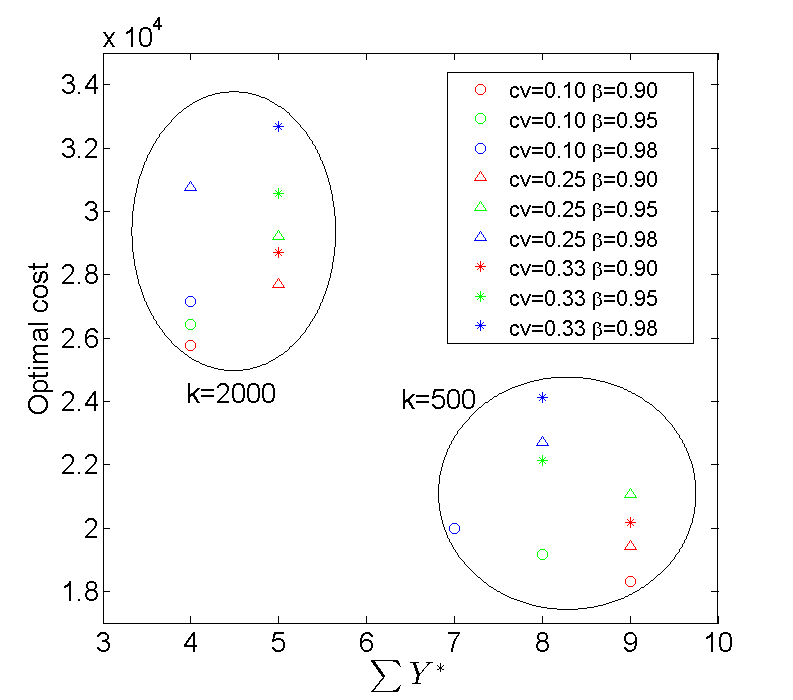
\includegraphics[scale=0.5]{iccsa2015/figures/experimentos.png}
%\includegraphics[scale=0.3]{qnbeta.pdf}
\caption{Optimal cost and number of ordering periods for every instance. Circles correspond to  $cv=0.10$, triangles to $cv=0.25$ and asterisks to $cv=0.33$. The values of $\beta=0.90$, $0.95$ and $0.98$ is represented by colors red, green and blue, respectively. $k$ identifies the ordering cost. Outcomes have been grouped according to the value of $k$.}
\label{fig:tests}
\end{figure}




With respect to efficiency, using Algorithm \ref{alg:optimalforYICCSA} (MinQ(Y)) instead of standard nonlinear optimization solver \emph{fmincon} reduces the computational time by a factor of 20. We specifically measured this for  Algorithm \ref{alg:bestYICCSA} without considering the existence of a lower bound function (line \ref{bestY:line:LB}), optimizing all feasible policies.  The main reason of the reduction is that MinQ(Y) uses all derived specific properties of the MINLP problem. 



\section{Conclusions}
\label{sec:conclusionsICCSA}
A MINLP model has been presented to determine order quantities for a perishable product inventory control problem. Basic order quantities can be determined to provide feasible production quantities for different delivery policies of the model. Theoretical properties of feasible order timings and of the NLP problem when the timing $Y$ is fixed have been derived. Based on that, a method has been developed to finding optimal quantities for the objective function (\ref{eq:objICCSA}) when the timing is given. For real applications, when $T$ is not very large, this method is able to find the optimal solution for the problem by exhaustive search of feasible policies, using a lower bound function on cost to reduce enumeration.
Moreover, obtained results have shown that the dedicated  method can reduce the runtime in a factor of $20$ with respect to the general purpose Matlab function \emph{fmincon} for solving NLP problems, while keeping the high quality of the optimal solutions.


As the NLP optimization given a timing vector $Y$ can be solved independently for each timing vector, a challenge for future investigation is to address the parallelization of the method. Such parallelization facilitates obtaining more accurate results due to a possible  increase of the number of Monte Carlo simulations to solve a particular problem and simultaneously reduces the runtime.




%--------------------------------------------------------------------------
%\section*{Appendix A: Description of the problems}
%\label{Sec:Ap}




%--------------------------------------------------------------------------
%
%\subsubsection*{Acknowledgments.}
%This paper has been supported by The Spanish Ministry  (TIN2012-37483) and Junta de Andaluc\'{\i}a (P11-TIC-7176), in part financed by the European Regional Development Fund (ERDF). The study is co-funded by the TIFN (project RE002).
%
%
%\begin{thebibliography}{1}
%\providecommand{\url}[1]{\texttt{#1}}
%\providecommand{\urlprefix}{URL }
%
%\bibitem{hedjar2004}
%Hedjar, R., Bounkhel, M., Tadj, L.: Predictive control of periodic-review
%  production inventory systems with deteriorating items. TOP  12(1),  193--208
%  (2004)
%
%\bibitem{HENTO10}
%Hendrix, E.M.T., Toth, B.G.: Introduction to Nonlinear and Global Optimization.
%  Springer, New York (2010)
%
%\bibitem{kurawarwala96}
%Kurawarwala, A.A., Matsuo, H.: Forecasting and inventory management of short
%  life-cycle products. Operations Research  44,  131--150 (1996)
%
%\bibitem{PAULS14}
%Pauls-Worm, K.G.J., Hendrix, E.M.T., Haijema, R., van~der Vorst, J.G.A.J.: An
%  {MILP} approximation for ordering perishable products with non-stationary
%  demand and service level constraints. International Journal of Production
%  Economics  157,  133--146 (2014)
%
%\bibitem{Rossi14}
%Rossi, R., Tarim, S.A., Prestwich, S., Hnich, B.: Piecewise linear lower and
%  upper bounds for the standard normal first order loss function. Applied
%  Mathematics and Computation  231,  489--502 (2014)
%
%\bibitem{Schrijver12}
%Schrijver, S.K.D., Aghezzaf, E.H., Vanmaele, H.: Double precision rational
%  approximation algorithm for the inverse standard normal first order loss
%  function. Applied Mathematics and Computation  219(3),  1375 -- 1382 (2012)
%
%\bibitem{Silver98}
%Silver, E.A., Pyke, D.F., Peterson, R.: Inventory Management and Production
%  Planning and Scheduling. Wiley (1998)
%
%\bibitem{Waissi96}
%Waissi, G.R., Rossin, D.F.: A sigmoid approximation of the standard normal
%  integral. Applied Mathematics and Computation  77(1),  91 -- 95 (1996)
%
%\end{thebibliography}
%
%
%\end{document}



%--------------------------------------------------------------------------
%\section*{Appendix A: Description of the problems}
%\label{Sec:Ap}
